\documentclass[a4paper,UTF8]{ctexart}

\usepackage{amsmath, amsthm, amssymb, amsfonts, hyperref, mathrsfs}%美国数学学会的包+?
\usepackage{geometry} %控制界面
\usepackage{bookmark}
\usepackage{fancyhdr} % header & footer
\usepackage{appendix} % 附录
\usepackage{tikz} %作图
\usepackage{graphicx} %插入图片的宏包
\usepackage{float} %设置图片浮动位置的宏包
\usepackage{subfigure} %插入多图时用子图显示的宏包
\usepackage{listings} %引用代码
\usepackage{physics,mathtools} %物理数学工具
\usepackage{framed}
\geometry{top=2.5cm,bottom=2.5cm,left=2.5cm,right=2.5cm} % 布局要求
\pagestyle{fancy} % fancy分格
\fancyhf{} % 清除所有页眉页脚
\renewcommand\headrulewidth{0.6pt}
\renewcommand\footrulewidth{0.6pt}
\lhead{何金铭 PB21020660$\mid$座位号:4}
\chead{磁阻效应实验数据处理}
\rhead{\thepage}
\lfoot{2022.11.24}
\rfoot{USTC}
%\bibliographystyle{plain} % 引用样式
\everymath{\displaystyle} % display
%============================================================

\begin{document}

\begin{center}
    \textbf{\Large 磁阻效应实验数据处理}
    \par \text{\large 何金铭 PB21020660}
\end{center}

\section{原始数据}

\subsection{一些基本数据}

\begin{description}
    \item[励磁系数 $\alpha$] $2400 Gs/A$
    \item[1,3方向的电阻$R_{13}$] $366.9 \Omega$
    \item[2,4方向的电阻$R_{24}$] $443.6 \Omega$
\end{description}

\subsection{电流方向为1,3方向,2,4方向断路,测量1,3方向电阻}

\begin{table}[!ht]
    \centering
    \begin{tabular}{|c|c|c|c|c|c|c|c|c|}
    \hline
        组数 & 1 & 2 & 3 & 4 & 5 & 6 & 7 & 8 \\ \hline
        $I / mA$ & 0 & 40 & 80 & 120 & 160 & 200 & 240 & 280 \\ \hline
        $R_1 / \Omega$ & 363.9 & 366.4 & 373.3 & 383.9 & 397.2 & 403.3 & 419.3 & 435.5 \\ \hline
        组数 & 9 & 10 & 11 & 12 & 13 & 14 & 15 & 16 \\ \hline
        $I / mA$ & 320 & 360 & 400 & 440 & 480 & 520 & 560 & 600 \\ \hline
        $R_1 / \Omega$ & 450.8 & 464.8 & 476.8 & 487.3 & 497.7 & 517.6 & 530.7 & 543.0 \\ \hline
        组数 & 17 & 18 & 19 & 20 & 21 & ~ & ~ & ~ \\ \hline
        $I / mA$ & 640 & 680 & 720 & 760 & 800 & ~ & ~ & ~ \\ \hline
        $R_1 / \Omega$ & 553.0 & 562.3 & 572.4 & 582.1 & 593.3 & ~ & ~ & ~ \\ \hline
    \end{tabular}
    \caption{$2,4$断路时的原始数据}
\end{table}

\subsection{电流方向为1,3方向,2,4方向短路,测量1,3方向电阻}

\begin{table}[!ht]
    \centering
    \begin{tabular}{|c|c|c|c|c|c|c|c|c|}
    \hline
        组数 & 1 & 2 & 3 & 4 & 5 & 6 & 7 & 8 \\ \hline
        $I / mA$ & 0 & 40 & 80 & 120 & 160 & 200 & 240 & 280 \\ \hline
        $R_1 / \Omega$ & 364.2 & 368.0 & 377.7 & 392.3 & 410.8 & 431.6 & 453.6 & 475.7 \\ \hline
        组数 & 9 & 10 & 11 & 12 & 13 & 14 & 15 & 16 \\ \hline
        $I / mA$ & 320 & 360 & 400 & 440 & 480 & 520 & 560 & 600 \\ \hline
        $R_1 / \Omega$ & 496.4 & 514.6 & 529.1 & 542.4 & 555.0 & 569.1 & 585.6 & 600.3 \\ \hline
        组数 & 17 & 18 & 19 & 20 & 21 & ~ & ~ & ~ \\ \hline
        $I / mA$ & 640 & 680 & 720 & 760 & 800 & ~ & ~ & ~ \\ \hline
        $R_1 / \Omega$ & 611.9 & 623.6 & 634.9 & 646.4 & 657.7 & ~ & ~ & ~ \\ \hline
    \end{tabular}
    \caption{$2,4$短路时的原始数据}
\end{table}

\subsection{电流方向为1,3方向,测量2,4方向电阻}

由于时间不够,未测量数据,只给出了测量方案,于下文中给出。

\section{实验方案}

\subsection{电流方向为1,3方向,2,4方向断路,测量1,3方向电阻}

对于励磁电路,使用$V=15v,I \in \left[0,0.8A\right]$的恒流源。

\begin{figure}[H]
    \centering
    \begin{minipage}[b]{0.9\textwidth}
        \centering
        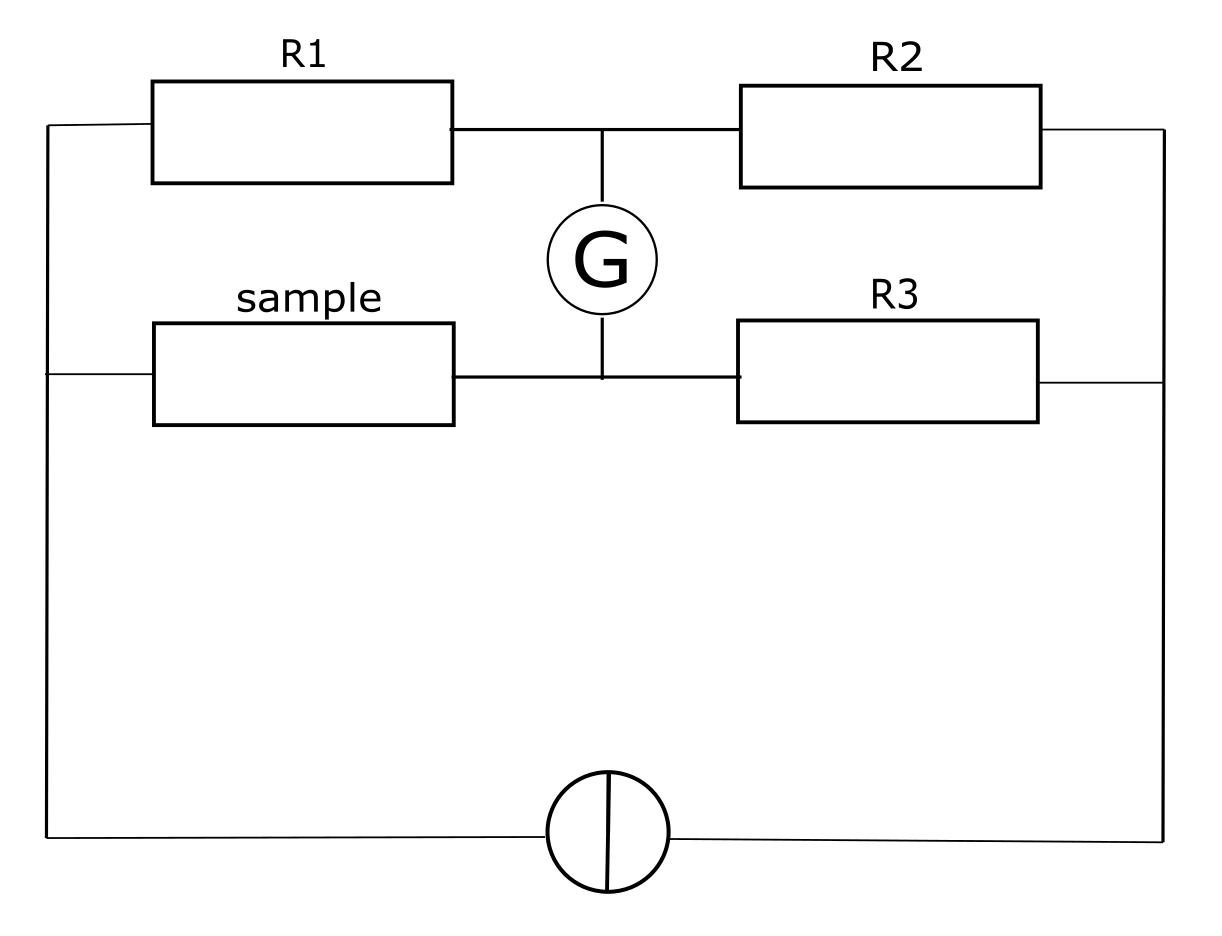
\includegraphics[width=0.7\textwidth]{./1.png}
        \caption{锑化铟片工作电流电路}
    \end{minipage}
\end{figure}

对于锑化铟片所在的电路,使用恒流源($I = 5 mA$)搭配平衡电桥电路进行测量,由于锑化铟片的电阻会随电流变化而变化,
所以选择固定$R_2,R_3$阻值不变,变化$R_1$,当$I_G$为0的时候,可以得到$R_{sample}=R_1$。

{\bfseries 实验方案}

于$0$到$0.8A$的范围内变化励磁电流,每次变化$0.04A$,每次调整微安表示数为0,记录下相应的$R_1$。

\subsection{电流方向为1,3方向,2,4方向短路,测量1,3方向电阻}

与上一个电路类似,唯一的区别是$2,4$回路处于短路状态。

\subsection{电流方向为1,3方向,测量2,4方向电阻}

\begin{figure}[H]
    \centering
    \begin{minipage}[b]{0.9\textwidth}
        \centering
        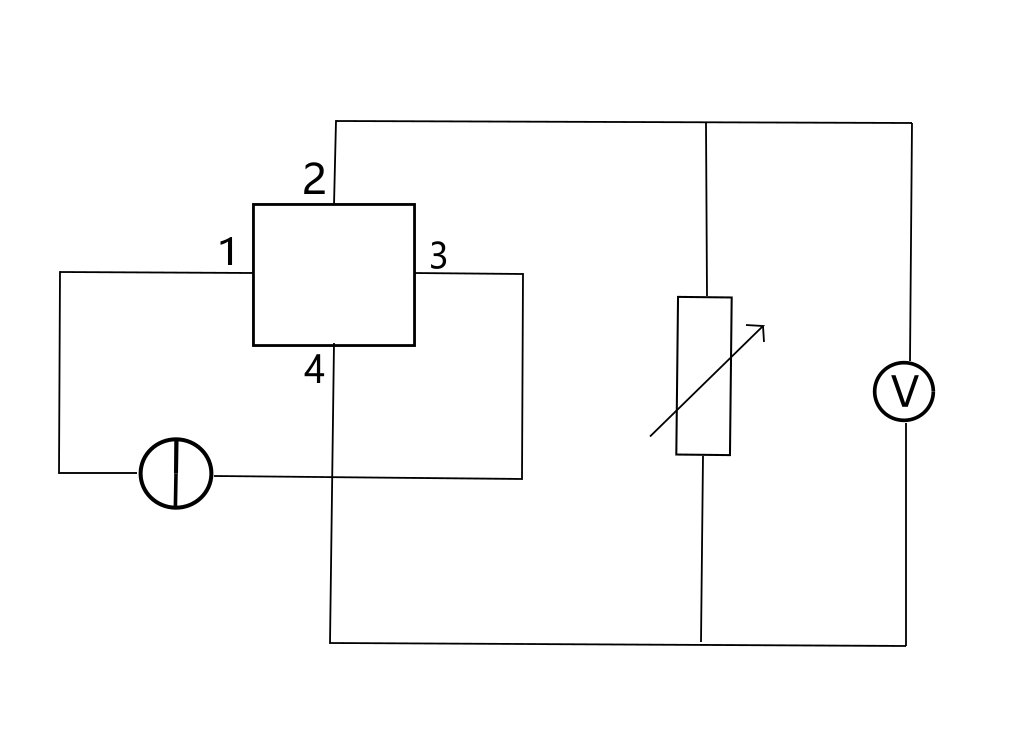
\includegraphics[width=0.7\textwidth]{./2.png}
        \caption{锑化铟片电路}
    \end{minipage}
\end{figure}

1,3方向为工作电流电路,2,4回路为测量电源内阻的回路。其中工作电路电流设定为$0.025 mA$

{\bfseries 实验方案}

于$0$到$0.8A$的范围内变化励磁电流,每次变化$0.05A$,对于每个励磁电流,改变5次电阻箱电阻,
记录下阻值$R$并记录相应的电压表示数$U$。

对于每一组的电阻和电压值进行拟合,

\begin{equation}
    \frac{1}{U} = \frac{r}{E} \cdot \frac{1}{R} + \frac{1}{E}
\end{equation}

获取拟合曲线$\frac{1}{U}$-$\frac{1}{R}$的截距和斜率,以此计算得$r$。

\section{数据处理}

通过公式

\begin{equation}
    B = \alpha \cdot I
\end{equation}

\begin{equation}
    \frac{\Delta R}{R(0)} = \frac{R-R(0)}{R(0)}
\end{equation}

可以计算得:$B$与$\frac{\Delta R}{R(0)}$,并作图。

\subsection{电流方向为1,3方向,2,4方向断路,测量1,3方向电阻}

\begin{figure}[H]
    \centering
    \begin{minipage}[b]{0.9\textwidth}
        \centering
        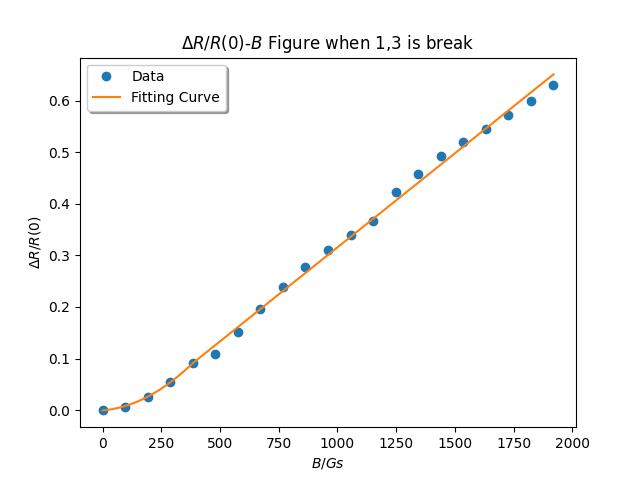
\includegraphics[width=0.7\textwidth]{./fig_1.png}
        \caption{2,4回路断路时的$\Delta R/R(0)$-$B$图}
    \end{minipage}
\end{figure}

{\bfseries 分析}

\begin{enumerate}
    \item 对于前五个数据$\Delta R/R(0)$正比于磁感应强度$B$的平方,与理论符合。
    \item 对于之后的数据$\Delta R/R(0)$与磁感应强度$B$呈线性关系,与理论符合。
\end{enumerate}

\subsection{电流方向为1,3方向,2,4方向短路,测量1,3方向电阻}

\begin{figure}[H]
    \centering
    \begin{minipage}[b]{0.9\textwidth}
        \centering
        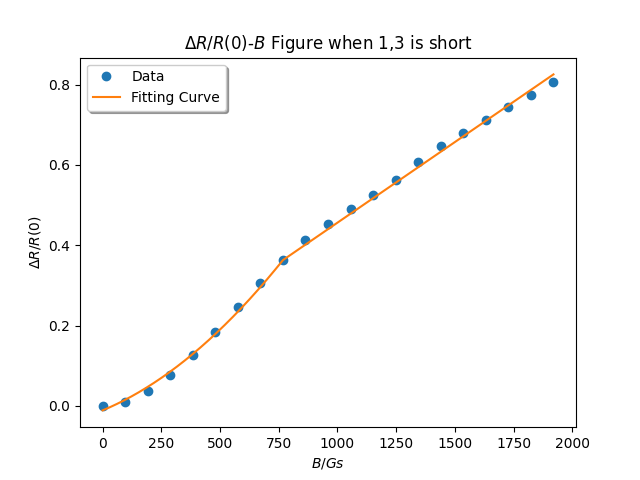
\includegraphics[width=0.7\textwidth]{./fig_2.png}
        \caption{2,4回路短路时的$\Delta R/R(0)$-$B$图}
    \end{minipage}
\end{figure}

{\bfseries 分析}

\begin{enumerate}
    \item 对于前9个数据$\Delta R/R(0)$正比于磁感应强度$B$的平方,与理论符合。
    \item 对于之后的数据$\Delta R/R(0)$与磁感应强度$B$呈线性关系,与理论符合。
    \item 且对比$2,4$短路与断路时的情况,发现当磁感应强度$B$相同的时候,$2,4$短路时的$\Delta R/R(0)$较$2,4$断路时的大,可知$2,4$短路时
    磁阻效应更明显,符合理论。
\end{enumerate}

\end{document}